\documentclass[10pt, compress, aspectratio=169]{beamer}

\usetheme[numbering=fraction, progressbar=none, titleformat=smallcaps]{metropolis}
\usepackage{booktabs}
\usepackage{array}
\usepackage{listings}
\usepackage{graphicx}
\usepackage[scale=2]{ccicons}
\usepackage{url}
\usepackage{relsize}
\usepackage{wasysym}

\usepackage{pgfplots}
\usepgfplotslibrary{dateplot}

\lstset{ %
  backgroundcolor={},
  basicstyle=\ttfamily\footnotesize,
  breakatwhitespace=true,
  breaklines=true,
  captionpos=n,
  commentstyle=\color{orange},
  escapeinside={\%*}{*)},
  extendedchars=true,
  frame=n,
  keywordstyle=\color{orange},
  language=bash,
  rulecolor=\color{black},
  showspaces=false,
  showstringspaces=false,
  showtabs=false,
  numbers=left,
  numbersep=3pt,
  stepnumber=1,
  stringstyle=\color{gray},
  tabsize=2,
  keywords={thrust,plus,device_vector, copy,transform,begin,end, copyin,
  copyout, acc, \_\_global\_\_, void, int, float, main, threadIdx, blockIdx,
  blockDim, if, else, malloc, NULL, cudaMalloc, cudaMemcpy, cudaSuccess,
  cudaGetLastError, cudaDeviceSynchronize, cudaFree, cudaMemcpyDeviceToHost,
  cudaMemcpyHostToDevice, const, data, independent, kernels, loop,
  fprintf, stderr, cudaGetErrorString, EXIT_FAILURE, for, dim3},
  otherkeywords={::, \#pragma, \#include, <<<,>>>, \&, \*, +, -, /, [, ], >, <}
}

\renewcommand*{\UrlFont}{\ttfamily\smaller\relax}

\graphicspath{{images/}}

\title{Using History Interactively}
\author{\footnotesize Rodrigo Siqueira \\ {\scriptsize siqueira@ime.usp.br}}
%\institute{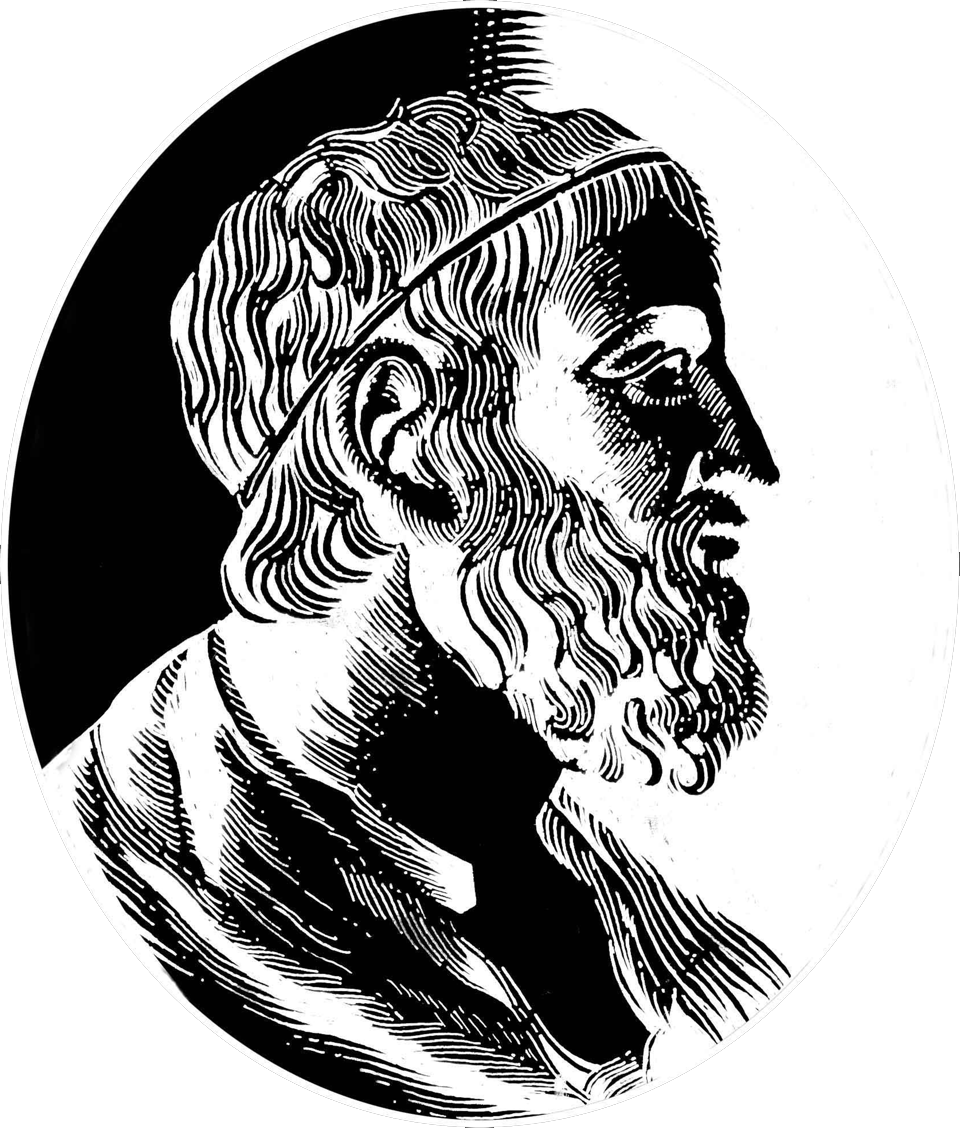
\includegraphics[height=2cm]{imelogo}\\[0.2cm] Department of Computer Science \\ University of São Paulo}

\begin{document}

\maketitle

%------------------------------------------------------------------------------
\section{Introduction}
\begin{frame}{Basic definitions}
  \metroset{block=fill}
  \begin{exampleblock}{Bases}
    \begin{itemize}
      \item Bash history stream can be dynamically edited
      \item Bash variables:
				\begin{itemize}
					\item \texttt{HISTSIZE}: History size
					\item \texttt{HISTFILE}: History file name
					\item \texttt{HISTTIMEFORMAT}: Format to save inside history
					\item \texttt{HISTCONTROL}: Control history behaviour. There is two
								useful contro: \texttt{ignoredups} and \texttt{erasedups}. The
								former makes bash not store repeated commands in a sequence and
								the letter remove duplications from the history
				\end{itemize}
    \end{itemize}
  \end{exampleblock}
\end{frame}

%------------------------------------------------------------------------------
\section{Bash History Builtins}

\begin{frame}{Builtins: \texttt{fc}}
  \metroset{block=fill}
  \begin{alertblock}{Syntax}
    \begin{itemize}
      \item \texttt{fc [-e ename] [-lnr] [first] [last]}
      \item \texttt{fc -s [pat=rep] [command]}
    \end{itemize}
  \end{alertblock}
\end{frame}

\begin{frame}{Builtins: \texttt{history}}
  \metroset{block=fill}
  \begin{alertblock}{Syntax}
    \begin{itemize}
      \item \texttt{history [n]}
      \item \texttt{history -c}
      \item \texttt{history -d offset}
      \item \texttt{history [-anrw] [filename]}
			\item \texttt{history -ps arg}
    \end{itemize}
  \end{alertblock}
\end{frame}

%------------------------------------------------------------------------------
\section{History Expansion}

\begin{frame}{History Expansion}
  \metroset{block=fill}
  \begin{exampleblock}{About}
    \begin{itemize}
      \item History expansion are based into two parts: \textit{words} and
						\textit{event}
			\item \textbf{event}: Point out the history line 
			\item \textbf{word}: Point out a part of the command in history
			\item \textbf{(event, word)}: Word and Event works like a coordinate
						system
    \end{itemize}
  \end{exampleblock}
\end{frame}

\begin{frame}{History Expansion: Event}
  \metroset{block=fill}
  \begin{exampleblock}{Basic designators}
    \begin{itemize}
			\item Represented by \texttt{!}
			\item Designators:
			\begin{itemize}
				\item \texttt{!n}: Command line n
				\item \texttt{!-n}: Command line back
				\item \texttt{!!}: Last command
				\item \texttt{!string}: Most recent command started with \texttt{string}
				\item \texttt{\^string1\^string2\^}: Replace string1 by string2 in the
							last command
			\end{itemize}
    \end{itemize}
  \end{exampleblock}
\end{frame}

\begin{frame}{History Expansion: Word}
  \metroset{block=fill}
  \begin{exampleblock}{Basic designators}
    \begin{itemize}
			\item Represented by \texttt{:}
			\item Designators:
			\begin{itemize}
				\item \texttt{!!:\textdollar{}}: Command line n
				\item \texttt{\^}: Command line back
				\item \texttt{\textdollar{}}: Last command
			\end{itemize}
    \end{itemize}
  \end{exampleblock}

  \begin{exampleblock}{Basic Modifiers}
    \begin{itemize}
			\item \texttt{h}: Remove a trailing pathname component
			\item \texttt{t}: Remove all pathname
			\item \texttt{r}: Remove trailing suffix
			\item \texttt{e}: Remove all but the trailing suffix
			\item \texttt{p}: print the new command but do not execute it
    \end{itemize}
  \end{exampleblock}

\end{frame}

%------------------------------------------------------------------------------
\section{About this presentation}
\begin{frame}[standout]
  % TODO: Improve it
   \begin{center}\ccbysa\end{center}
\end{frame}

%TODO: Bibliography
% break [n]: http://tldp.org/LDP/abs/html/loopcontrol.html
% continue [n]: http://tldp.org/LDP/abs/html/loopcontrol.html
% exec: http://wiki.bash-hackers.org/commands/builtin/exec
% caller: http://wiki.bash-hackers.org/commands/builtin/caller
% key num code: http://invisible-island.net/xterm/xterm-function-keys.html
\maketitle

\end{document}
